%%%%%%%%%%%%%%%%%%%%%%%%%%%%%%%%%%%%%%%%%%%%%%%%%%%%%%%%%%%%%%%%%%%%%%%%%%%%%%%%
% Template for USENIX papers.
%
% History:
%
% - TEMPLATE for Usenix papers, specifically to meet requirements of
%   USENIX '05. originally a template for producing IEEE-format
%   articles using LaTeX. written by Matthew Ward, CS Department,
%   Worcester Polytechnic Institute. adapted by David Beazley for his
%   excellent SWIG paper in Proceedings, Tcl 96. turned into a
%   smartass generic template by De Clarke, with thanks to both the
%   above pioneers. Use at your own risk. Complaints to /dev/null.
%   Make it two column with no page numbering, default is 10 point.
%
% - Munged by Fred Douglis <douglis@research.att.com> 10/97 to
%   separate the .sty file from the LaTeX source template, so that
%   people can more easily include the .sty file into an existing
%   document. Also changed to more closely follow the style guidelines
%   as represented by the Word sample file.
%
% - Note that since 2010, USENIX does not require endnotes. If you
%   want foot of page notes, don't include the endnotes package in the
%   usepackage command, below.
% - This version uses the latex2e styles, not the very ancient 2.09
%   stuff.
%
% - Updated July 2018: Text block size changed from 6.5" to 7"
%
% - Updated Dec 2018 for ATC'19:
%
%   * Revised text to pass HotCRP's auto-formatting check, with
%     hotcrp.settings.submission_form.body_font_size=10pt, and
%     hotcrp.settings.submission_form.line_height=12pt
%
%   * Switched from \endnote-s to \footnote-s to match Usenix's policy.
%
%   * \section* => \begin{abstract} ... \end{abstract}
%
%   * Make template self-contained in terms of bibtex entires, to allow
%     this file to be compiled. (And changing refs style to 'plain'.)
%
%   * Make template self-contained in terms of figures, to
%     allow this file to be compiled. 
%
%   * Added packages for hyperref, embedding fonts, and improving
%     appearance.
%   
%   * Removed outdated text.
%
%%%%%%%%%%%%%%%%%%%%%%%%%%%%%%%%%%%%%%%%%%%%%%%%%%%%%%%%%%%%%%%%%%%%%%%%%%%%%%%%

\documentclass[letterpaper,twocolumn,10pt]{article}
\usepackage{usenix2019_v3}

% to be able to draw some self-contained figs
\usepackage{tikz}
\usepackage{amsmath}
\usepackage{cite}

% inlined bib file
\usepackage{filecontents}


%-------------------------------------------------------------------------------
\begin{document}
%-------------------------------------------------------------------------------

%don't want date printed
\date{}

% make title bold and 14 pt font (Latex default is non-bold, 16 pt)
\title{\Large \bf Reduce Performance Impact of Compaction Process by Designing a Global Format for LSM}

%for single author (just remove % characters)
\author{
{\rm Jinghuan YU}\\
City University of Hong Kong
\and
{\rm Chun Jason. Xue}\\
City University of Hong Kong
} % end author

\maketitle

%-------------------------------------------------------------------------------
\begin{abstract}
%-------------------------------------------------------------------------------
Your abstract text goes here. Just a few facts. Whet our appetites.
Not more than 200 words, if possible, and preferably closer to 150.
\end{abstract}


%-------------------------------------------------------------------------------
\section{Introduction}
%-------------------------------------------------------------------------------

\section{Background}
\textbf{\textit{ Some Quick Conclusion HERE}}

\subsection{Non-Volatile Memory}
NVM, or PM (persistent memory), SCM (storage class memory), is actually the same meaning, referring to a series of memory materials with non-volatile and byte-wise access characteristics. NVM has became a hot topic in recent years, and related research is moving forward. There are many different types materials like PCM (phase change memory), MRAM (Magnetoresistive RAM) etc. Beside the most obvious feature, NVM has higher throughput and storage density than traditional NAND flash devices, with the shortages like asymmetrical read/write performance, and limited lifetime leads to the wear-out problems.

%\paragraph{Typical Usage of NVM in Practice} 

Although there is no final conclusion on how to use this material, research proposed several main solutions for using this material: 

1. Use NVM as Persistent Transnational Memory, use methods like Redo Logging, Undo Logging, and Log-Structured to manage the transaction and data involved. 

2. Use NVM as a disk to provide better random access performance on blocks and files. For example, introducing the Direct Access (DAX) in Linux. There are also file systems\cite{dulloor2014system} similar to PMFS, NOVA\cite{xu2016nova}, etc.

3. Combining with RDMA in a distributed scenario. Due to the high performance of NVM, the access characteristics of byte addressing, and the access mode of RDMA, distributed NVM + RDMA becomes a new architecture design.


\subsection{Log-Structured-Merged Tree}\label{LSM-introduction}
LSM Tree is a high warm writing performance data structure proposed in 1996\cite{o1996log}, gets widely used in many products like  Cassandra\cite{ApacheCa22:online}, Hbase\cite{ApacheHB26:online}, BigTable\cite{chang2008bigtable} and WiredTiger\cite{WiredTig38:online}.  The most important characteristics LSM has are sequential write optimized and its periodic garbage collection.

\subsubsection{Sequential Write Optimized} 

LSM's basic idea is converting random writes to sequential writes. Most of the storage devices has the characteristics that can perform much better in sequential operations than in random access operations, no matter read or write. LSM caches the newest changes inside the memory and use batch processing to write down those cached data. In addition to simply aggregate the operations, recent updated data will overwrite in
memory and be flash to the file system only for the last version.

\subsubsection{Periodic Garbage Collection} 

For using log-structure and incremental update to persistent operations. Data stored may be outdated periodically due to deletions and updates, so garbage collection process known as ``Compaction'' is needed. During the compaction process, LSM-based system will iterate through part of the persistent data, delete the out-dated data and reorganize the data in partial sorted manner to keep read optimal.

For this \textit{Compaction} process will walk through all key-value pairs stored in the target files, apply merge sorting to these entries and write back to the files. Though most of implementations tried to optimize compaction process, there are still very severe performance impact and resource occupying problems during this process. Fig. \ref{fig:disk_usage} shows the disk usage over time. These problems have been studied from many years ago, there are three main directions to solve these problems. 

\begin{figure}
	\centering
	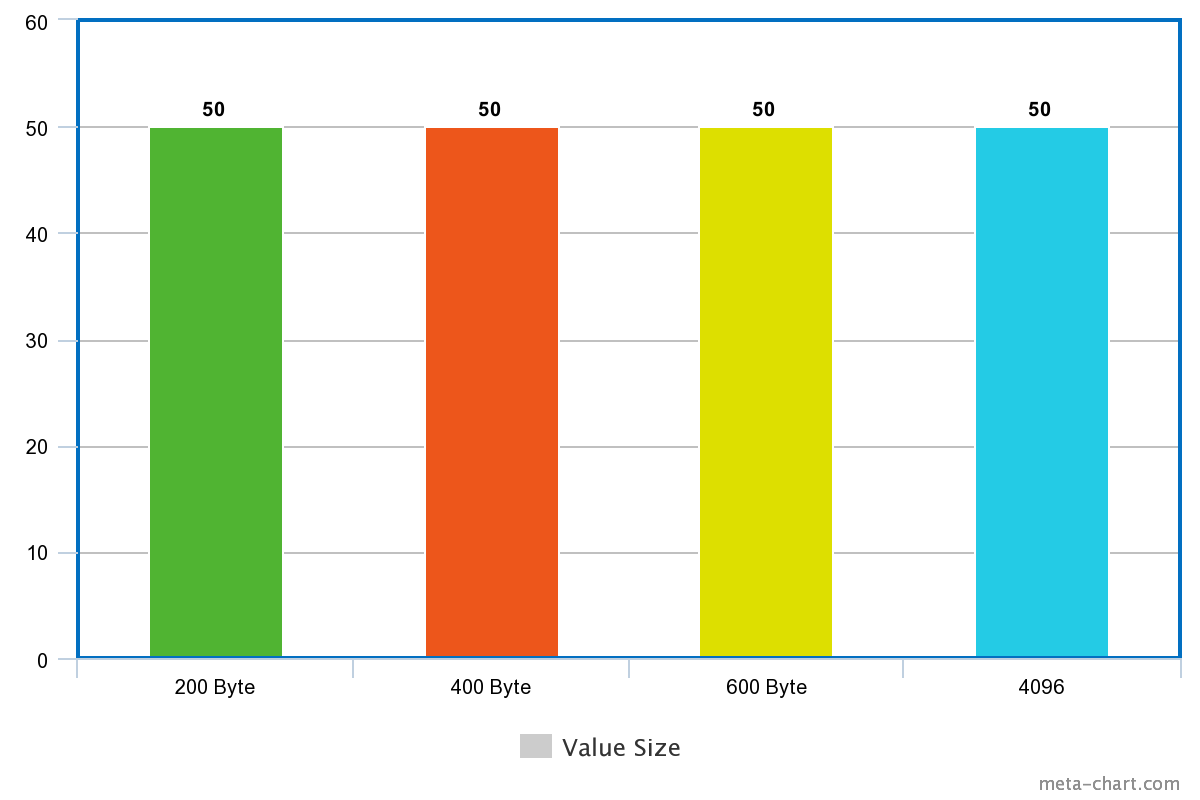
\includegraphics[width=0.7\columnwidth]{fig/meta-chart}
	\caption{This chart shows the sudden increasing disk usage while system fall into compaction.}
	\label{fig:disk_usage}
\end{figure}

\begin{itemize}
	\item The first one is \textbf{scheduling},  bLSM\cite{sears2012blsm} proposed a ``Gear Scheduler'' to dispersion pressure caused by compaction. It inspired many following works and most of the work mentioned in this paper used bLSM's results as base line while discussing scheduling problems. 
	\item 
	The second one is \textbf{algorithm optimization}, the most successful and representative one is PebblesDB in 2017\cite{raju2017pebblesdb}, use ``Guard'' to avoid repeated writing entries into files, easing the pressure by reducing write amplification. There are also works focus on special workloads like LSM-trie\cite{wu2015lsm}. And this may be the most popular thoughts in practice, Facebook provides several different types of compaction in RocksDB\cite{Compacti60:online},\cite{dong2017optimizing} while Cassandra also changed many times for its compaction strategy\cite{Document20:online}.  
	\item The third one is about \textbf{takeing advantages of new storage materials}, for new materials has been developed lot recent years, how these new materials', like Open-Channel SSD\cite{bjorling2017lightnvm} and NVM, characteristics may benefit the LSM data structure becomes a attractive topic to develop. GearDB\cite{yao2019geardb} considered reorganizing the entries choosing strategy to cover the garbage collection on HM-SMR disks. FlashKV\cite{zhang2017flashkv} use Open-Channel SSDs to optimize the compaction process's write amplification, achieved higher GC-efficiency. Novelsm\cite{kannan2018redesigning} utilized the characteristics of NVM's byte-addressing to achieve in-place update while SLM-DB\cite{kaiyrakhmet2019slm} combined with persistent B-Tree to organize the files into one single level and use \textit{select-merging} to get better performance in compaction.
	
\end{itemize}

\subsection{Chances and Challenges}
Programming for NVM is very different from traditional memory or disk programming, this section describes several main challenges while combing the NVM with the LSM structures.

\subsubsection{Space Amplification}
Fundamentally, this problem is unavoidable for any log-based system as the trade off for update costs and point looking up costs. Some hardware devices like HM-SMR and Open-channel may provide raw disk control to the applications, make it is possible for application to cover this problem with device's own garbage collection process\cite{zhang2017flashkv}.

\begin{figure}
	\centering
	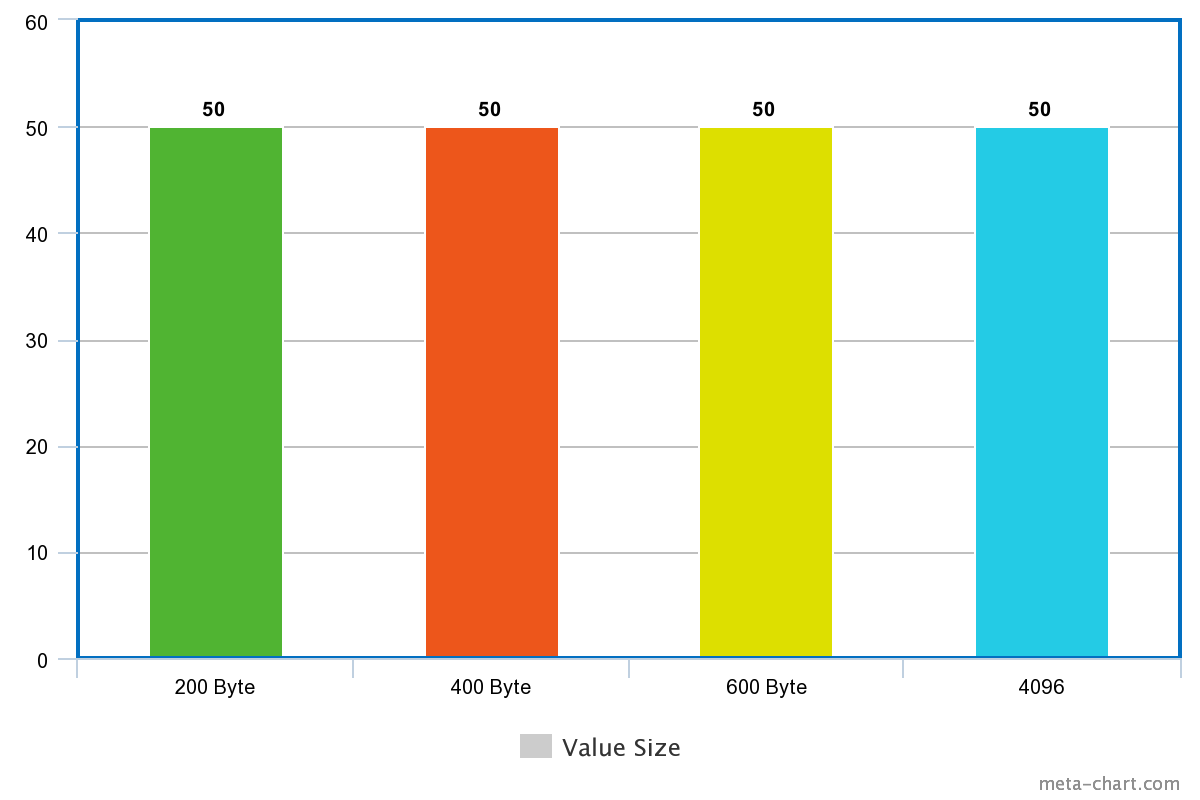
\includegraphics[width=0.7\columnwidth]{fig/meta2}
	\caption{The introduce of space amplification, the different reasons' ratio in entire result, point out most of the amplification problem is caused by the Compaction}
	\label{fig:space_amplification}
\end{figure}

This problem can be the most typical shortage of LSM-based systems, PepplesDB\cite{raju2017pebblesdb} and RocksDB\cite{dong2017optimizing} tried to solve this problem by optimizing the write down process, while Novelsm\cite{kannan2018redesigning} applied in-place updates on NVM to reduce repeated writing and SLM-DB use persistent B-Tree to solve this problem.

NVM's byte addressing ability allows more flexible data structure and operations; Its large capacity also benefits the buffer to store much more data, caching more operations before writing down to the sequential-based devices. This can reduce space amplification from the very origin purpose.

\subsubsection{Consistency}

the most important is the consistency problem. For example, consider about the situation of double-linked table insert operation, while the following code executes to the second line and meets a sudden power failure.
\begin{verbatim}
void list_add_tail(struct cds_list_head *newp,
struct cds_list_head *head) {
	head->prev->next = newp;
	newp->next = head;
	newp->prev = head->prev;
	head->prev = newp;
}
\end{verbatim}
For it is non-volatile in the NVM, when the system is restored, the linked list is in an abnormal state caused by the CPU Cache and the out-of-order execution of CPU. This means NVM requires a specified \textit{transaction programming} model\cite{dulloor2014system,ren2015thynvm} to ensure the semantics of atomic operations are achieved, which means there is no intermediate state generated during the system is restoring, this results in the extra memory fence and cache flush operations to keep consistency. Moreover, to provide consistent writing on data blocks larger than limited size (8 bytes in typical situations), logging and C-o-W (Copy on Write) is needed.

\subsubsection{Frequent serialization and de-serialization}

LSM system achieved buffering data inside memory to provide append-only writing strategy, and many of implementations use \textit{MemTable} as in-memory buffer and \textit{SST} (Sorted String Table) files to store Key-Value pairs in the file system. 

Use LevelDB\cite{LevelDBo44:online} as an example, while applying a \textit{Get} operation, LevelDB will first find in the memory buffer (\textit{Memtable}), then access the version control to check which file contains the target key-value pair; After locating the file, it still needs use several iterator to transfer the file blocks to memory structure, and decode from pre-compression format to get the real value. 

\begin{figure}
	\centering
	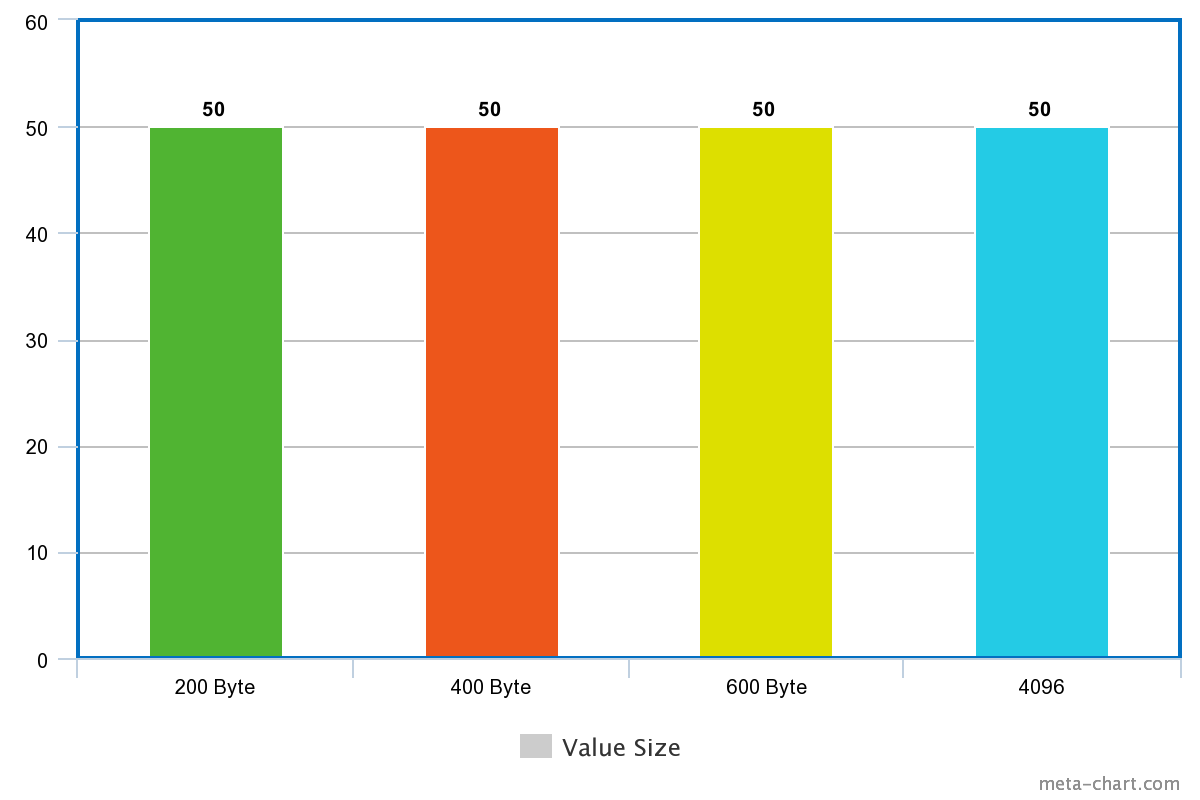
\includegraphics[width=0.7\columnwidth]{fig/meta-chart}
	\caption{This chart shows the ratio of time used on reading file block from disk during compaction.}
	\label{fig:file_read_ratio}
\end{figure}

\textbf{Fig. \ref{fig:file_read_ratio} shows a result that is not so common sense, the time spent on serialization and de-serialization take the most part of the system, much higher than the time spent on reading file blocks.}

\section{Proposed Solution}
The challenge is to design a LSM-based system with only one single data structure which can serve both inside the memory space and 
\subsubsection{}


%-------------------------------------------------------------------------------
\bibliographystyle{plain}
\bibliography{main}

%%%%%%%%%%%%%%%%%%%%%%%%%%%%%%%%%%%%%%%%%%%%%%%%%%%%%%%%%%%%%%%%%%%%%%%%%%%%%%%%
\end{document}
%%%%%%%%%%%%%%%%%%%%%%%%%%%%%%%%%%%%%%%%%%%%%%%%%%%%%%%%%%%%%%%%%%%%%%%%%%%%%%%%

%%  LocalWords:  endnotes includegraphics fread ptr nobj noindent
%%  LocalWords:  pdflatex acks
